%\VignetteIndexEntry{The quantro user's guide}
%\VignettePackage{quantro}
%\VignetteEngine{knitr::knitr}
\documentclass{article}\usepackage[]{graphicx}\usepackage[usenames,dvipsnames]{color}
%% maxwidth is the original width if it is less than linewidth
%% otherwise use linewidth (to make sure the graphics do not exceed the margin)
\makeatletter
\def\maxwidth{ %
  \ifdim\Gin@nat@width>\linewidth
    \linewidth
  \else
    \Gin@nat@width
  \fi
}
\makeatother

\definecolor{fgcolor}{rgb}{0.345, 0.345, 0.345}
\newcommand{\hlnum}[1]{\textcolor[rgb]{0.686,0.059,0.569}{#1}}%
\newcommand{\hlstr}[1]{\textcolor[rgb]{0.192,0.494,0.8}{#1}}%
\newcommand{\hlcom}[1]{\textcolor[rgb]{0.678,0.584,0.686}{\textit{#1}}}%
\newcommand{\hlopt}[1]{\textcolor[rgb]{0,0,0}{#1}}%
\newcommand{\hlstd}[1]{\textcolor[rgb]{0.345,0.345,0.345}{#1}}%
\newcommand{\hlkwa}[1]{\textcolor[rgb]{0.161,0.373,0.58}{\textbf{#1}}}%
\newcommand{\hlkwb}[1]{\textcolor[rgb]{0.69,0.353,0.396}{#1}}%
\newcommand{\hlkwc}[1]{\textcolor[rgb]{0.333,0.667,0.333}{#1}}%
\newcommand{\hlkwd}[1]{\textcolor[rgb]{0.737,0.353,0.396}{\textbf{#1}}}%

\usepackage{framed}
\makeatletter
\newenvironment{kframe}{%
 \def\at@end@of@kframe{}%
 \ifinner\ifhmode%
  \def\at@end@of@kframe{\end{minipage}}%
  \begin{minipage}{\columnwidth}%
 \fi\fi%
 \def\FrameCommand##1{\hskip\@totalleftmargin \hskip-\fboxsep
 \colorbox{shadecolor}{##1}\hskip-\fboxsep
     % There is no \\@totalrightmargin, so:
     \hskip-\linewidth \hskip-\@totalleftmargin \hskip\columnwidth}%
 \MakeFramed {\advance\hsize-\width
   \@totalleftmargin\z@ \linewidth\hsize
   \@setminipage}}%
 {\par\unskip\endMakeFramed%
 \at@end@of@kframe}
\makeatother

\definecolor{shadecolor}{rgb}{.97, .97, .97}
\definecolor{messagecolor}{rgb}{0, 0, 0}
\definecolor{warningcolor}{rgb}{1, 0, 1}
\definecolor{errorcolor}{rgb}{1, 0, 0}
\newenvironment{knitrout}{}{} % an empty environment to be redefined in TeX

\usepackage{alltt}

\RequirePackage{/Library/Frameworks/R.framework/Versions/3.1/Resources/library/BiocStyle/resources/latex/Bioconductor}

\AtBeginDocument{\bibliographystyle{/Library/Frameworks/R.framework/Versions/3.1/Resources/library/BiocStyle/resources/latex/unsrturl}}


\setlength{\parskip}{1\baselineskip}
\setlength{\parindent}{0pt}

\title{The \texttt{quantro} user's guide}
\author{Stephanie C. Hicks \texttt{shicks@jimmy.harvard.edu} \and
Rafael A. Irizarry \texttt{rafa@jimmy.harvard.edu} }

\date{Modified: March 24, 2015.  Compiled: \today}
\IfFileExists{upquote.sty}{\usepackage{upquote}}{}
\begin{document}

\maketitle
 
\tableofcontents

\section{Introduction}

Multi-sample normalization techniques such as quantile normalization 
\cite{Bolstad2003, Irizarry2003} have become a standard and essential part of 
analysis pipelines for high-throughput data. Although it was originally 
developed for gene expression microarrays, it is now used across many 
different high-throughput applications including genotyping arrays, DNA 
Methylation, RNA Sequencing (RNA-Seq) and Chromatin Immunoprecipitation 
Sequencing (ChIP-Seq). These techniques transform the original raw data to 
remove unwanted technical variation. However, quantile normalization and other 
global normalization methods rely on assumptions about the data generation 
process that are not appropriate in some context. Until now, it has been left 
to the researcher to check for the appropriateness of these assumptions. 

Quantile normalization assumes that the statistical distribution of each 
sample is the same. Normalization is achieved by forcing the observed 
distributions to be the same and the average distribution, obtained by taking 
the average of each quantile across samples, is used as the reference. This 
method has worked very well in practice but note that when the assumptions are 
not met, global changes in distribution, that may be of biological interest, 
will be wiped out and features that are not different across samples can be 
artificially induced.  These types of assumptions are justified in many 
biomedical applications, for example in gene expression studies in which only 
a minority of genes are expected to be differentially expressed. However, if, 
for example, a substantially higher percentage of genes are expected to be 
expressed in only one group of samples, it may not be appropriate to use 
global adjustment methods. 

The \texttt{quantro} R-package can be used to test for global differences 
between groups of distributions which asses whether global normalization 
methods such as quantile normalization should be applied. Our method uses 
the raw unprocessed high-throughput data to test for global differences in 
the distributions across a set of groups. The main function \texttt{quantro()} 
will perform two tests: 

\begin{enumerate} 

\item An ANOVA to test if the medians of the distributions are different 
across groups. Differences across groups could be attributed to unwanted 
technical variation (such as batch effects) or real global biological 
variation. This is a helpful step for the user to verify if there is any 
technical variation unaccounted for. 

\item A test for global differences between the distributions across groups 
which returns a test statistic called \texttt{quantroStat}. This test 
statistic is a ratio of two variances and is similar to the idea of ANOVA. 
The main idea is to compare the variability of distributions within groups 
relative to between groups. If the variability between groups is sufficiently 
larger than the variability within groups, then this suggests global 
adjustment methods may not be appropriate. As a default, we perform this test 
on the median normalized data, but the user may change this option. 

\end{enumerate}



\section{Getting Started}

Load the package in R

\begin{knitrout}
\definecolor{shadecolor}{rgb}{0.969, 0.969, 0.969}\color{fgcolor}\begin{kframe}
\begin{alltt}
\hlkwd{library}\hlstd{(quantro)}
\end{alltt}
\end{kframe}
\end{knitrout}

\section{Data}

\subsection{flowSorted Data Example}
To explore how to use \texttt{quantro()}, we use the 
\texttt{FlowSorted.DLPFC.450k} data package in Bioconductor 
\cite{JaffeFlowSorted}.  This data set contains raw data objects of 58 
Illumina 450K DNA methylation microarrays, formatted as \texttt{RGset} 
objects. The samples represent two different cellular populations of brain 
tissues on the same 29 individuals extracted using flow sorting.  For more 
information on this data set, please see the FlowSorted.DLPFC.450k User's 
Guide.  For the purposes of this vignette, a MethylSet object from the 
\texttt{minfi} Bioconductor package \cite{Aryee2014} was created which is 
a subset of the rows from the original \texttt{FlowSorted.DLPFC.450k} data 
set. This MethylSet object is found in the /data folder and the script to 
create the object is found in /inst.  

Here we will explore the distributions of these two cellular populations of 
brain tissue (\verb+NeuN_pos+ and \verb+NeuN_neg+) and then test if there 
are global differences in the distributions across groups. First, load the 
MethylSet object (\texttt{flowSorted}) and compute the Beta values using 
the function \texttt{getBeta()} in the \texttt{minfi} Bioconductor package. 
We use an offset of 100 as this is the default used by Illumina. 

\begin{knitrout}
\definecolor{shadecolor}{rgb}{0.969, 0.969, 0.969}\color{fgcolor}\begin{kframe}
\begin{alltt}
\hlkwd{library}\hlstd{(quantro)}
\hlkwd{library}\hlstd{(minfi)}
\hlkwd{data}\hlstd{(flowSorted)}
\hlstd{p} \hlkwb{<-} \hlkwd{getBeta}\hlstd{(flowSorted,} \hlkwc{offset} \hlstd{=} \hlnum{100}\hlstd{)}
\hlstd{pd} \hlkwb{<-} \hlkwd{pData}\hlstd{(flowSorted)}
\hlkwd{dim}\hlstd{(p)}
\end{alltt}
\begin{verbatim}
## [1] 10000    58
\end{verbatim}
\begin{alltt}
\hlkwd{head}\hlstd{(pd)}
\end{alltt}
\begin{verbatim}
##        Sample_Name SampleID CellType Sentrix.Barcode Sample.Section    diag    sex
## 813_N        813_N      813 NeuN_pos      7766130090         R02C01 Control Female
## 1740_N      1740_N     1740 NeuN_pos      7766130090         R02C02 Control Female
## 1740_G      1740_G     1740 NeuN_neg      7766130090         R04C01 Control Female
## 1228_G      1228_G     1228 NeuN_neg      7766130090         R04C02 Control   Male
## 813_G        813_G      813 NeuN_neg      7766130090         R06C01 Control Female
## 1228_N      1228_N     1228 NeuN_pos      7766130090         R06C02 Control   Male
##        ethnicity age PMI
## 813_N  Caucasian  30  14
## 1740_N   African  13  17
## 1740_G   African  13  17
## 1228_G Caucasian  47  13
## 813_G  Caucasian  30  14
## 1228_N Caucasian  47  13
##                                                                     BasePath
## 813_N  /dcs01/lieber/ajaffe/450k/Zack_450k/IDAT/7766130090/7766130090_R02C01
## 1740_N /dcs01/lieber/ajaffe/450k/Zack_450k/IDAT/7766130090/7766130090_R02C02
## 1740_G /dcs01/lieber/ajaffe/450k/Zack_450k/IDAT/7766130090/7766130090_R04C01
## 1228_G /dcs01/lieber/ajaffe/450k/Zack_450k/IDAT/7766130090/7766130090_R04C02
## 813_G  /dcs01/lieber/ajaffe/450k/Zack_450k/IDAT/7766130090/7766130090_R06C01
## 1228_N /dcs01/lieber/ajaffe/450k/Zack_450k/IDAT/7766130090/7766130090_R06C02
\end{verbatim}
\end{kframe}
\end{knitrout}




\subsection{Plot distributions}
\texttt{quantro} contains two functions to view the distributions of the 
samples of interest: \texttt{matdensity()} and \texttt{matboxplot()}. 
\texttt{matdensity()} computes the density for each sample (columns) and 
uses the \texttt{matplot()} function to plot all the densities. 
\texttt{matboxplot()} orders and colors the samples by a group level variable. 
These two functions use the \texttt{RColorBrewer} package and the brewer 
palettes can be changed using the arguments \texttt{brewer.n} and 
\texttt{brewer.name}. 

The distributions of the two groups of cellular populations are shown here. 
The \verb+NeuN_neg+ samples are colored in green and the \verb+NeuN_pos+ are 
colored in red.  

\begin{knitrout}
\definecolor{shadecolor}{rgb}{0.969, 0.969, 0.969}\color{fgcolor}\begin{kframe}
\begin{alltt}
\hlkwd{matdensity}\hlstd{(p,} \hlkwc{groupFactor} \hlstd{= pd}\hlopt{$}\hlstd{CellType,} \hlkwc{xlab} \hlstd{=} \hlstr{" "}\hlstd{,} \hlkwc{ylab} \hlstd{=} \hlstr{"density"}\hlstd{,}
           \hlkwc{main} \hlstd{=} \hlstr{"Beta Values"}\hlstd{,} \hlkwc{brewer.n} \hlstd{=} \hlnum{8}\hlstd{,} \hlkwc{brewer.name} \hlstd{=} \hlstr{"Dark2"}\hlstd{)}
\hlkwd{legend}\hlstd{(}\hlstr{'top'}\hlstd{,} \hlkwd{c}\hlstd{(}\hlstr{"NeuN_neg"}\hlstd{,} \hlstr{"NeuN_pos"}\hlstd{),} \hlkwc{col} \hlstd{=} \hlkwd{c}\hlstd{(}\hlnum{1}\hlstd{,} \hlnum{2}\hlstd{),} \hlkwc{lty} \hlstd{=} \hlnum{1}\hlstd{,} \hlkwc{lwd} \hlstd{=} \hlnum{3}\hlstd{)}
\end{alltt}
\end{kframe}
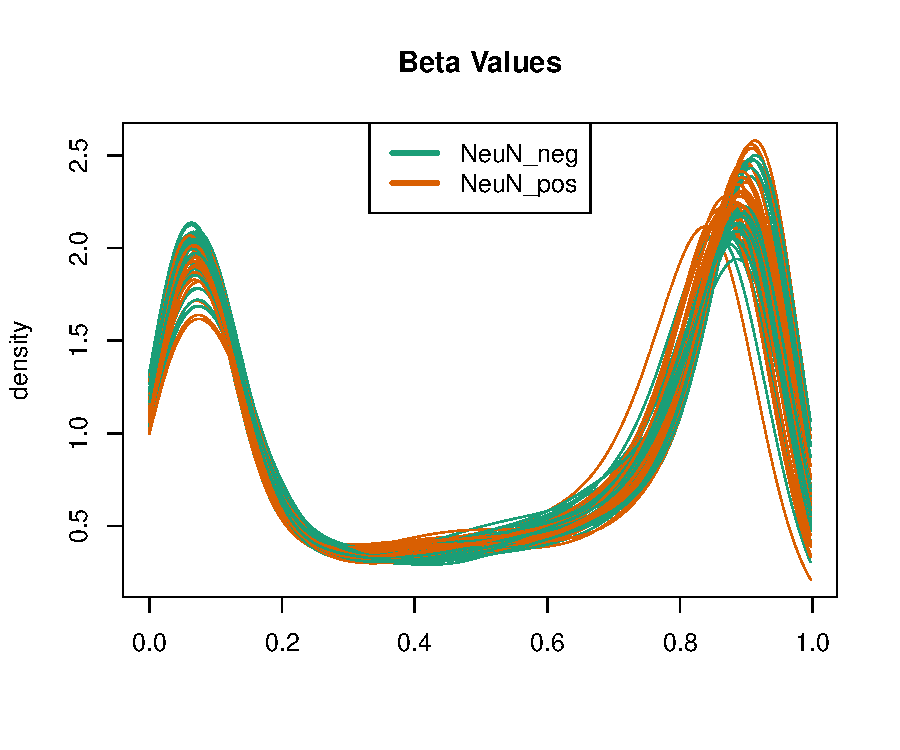
\includegraphics[width=\maxwidth]{figure/plot-distributions-density-1} 

\end{knitrout}


\begin{knitrout}
\definecolor{shadecolor}{rgb}{0.969, 0.969, 0.969}\color{fgcolor}\begin{kframe}
\begin{alltt}
\hlkwd{matboxplot}\hlstd{(p,} \hlkwc{groupFactor} \hlstd{= pd}\hlopt{$}\hlstd{CellType,} \hlkwc{xaxt} \hlstd{=} \hlstr{"n"}\hlstd{,} \hlkwc{main} \hlstd{=} \hlstr{"Beta Values"}\hlstd{)}
\end{alltt}
\end{kframe}
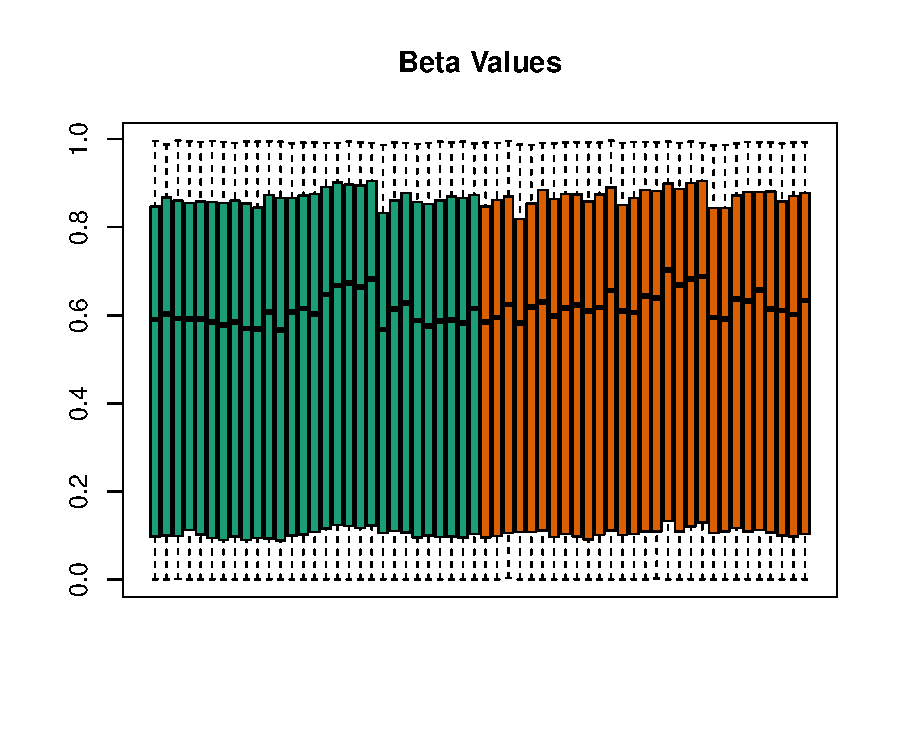
\includegraphics[width=\maxwidth]{figure/plot-distributions-boxplot-1} 

\end{knitrout}





\section{Using the \texttt{quantro()} function}

\subsection{Input for \texttt{quantro()}}
The \texttt{quantro()} function must have two objects as input: 

\begin{itemize}
\item an \texttt{object} which is a data frame or matrix with observations 
(e.g. probes or genes) on the rows and samples as the columns. 

\item a \texttt{groupFactor} which represents the group level information 
about each sample. For example if the samples represent tumor and normal 
samples, provide \texttt{quantro()} with a factor representing which columns 
in the \texttt{object} are normal and tumor samples.
\end{itemize}




\subsection{Running \texttt{quantro()}}
In this example, the groups we are interested in comparing are contained in 
the \texttt{CellType} column in the \texttt{pd} dataset. To run the 
\texttt{quantro()} function, input the data object and the object containing 
the phenotypic data. Here we use the \texttt{flowSorted} data set as an 
example. 

\begin{knitrout}
\definecolor{shadecolor}{rgb}{0.969, 0.969, 0.969}\color{fgcolor}\begin{kframe}
\begin{alltt}
\hlstd{qtest} \hlkwb{<-} \hlkwd{quantro}\hlstd{(}\hlkwc{object} \hlstd{= p,} \hlkwc{groupFactor} \hlstd{= pd}\hlopt{$}\hlstd{CellType)}
\end{alltt}


{\ttfamily\noindent\itshape\color{messagecolor}{\#\# [quantro] Average medians of the distributions are \\\#\#\ \ \ \ \ \ \ \ \ \ \ \ \ \ \ \ \ \ \ \ \ \ \ \  not equal across groups.\\\#\# [quantro] Calculating the quantro test statistic.\\\#\# [quantro] No permutation testing performed. \\\#\#\ \ \ \ \ \ \ \ \ \ \ \ \ \ \ \ \ \ \ \ \ \ \ \ \ \ Use B > 0 for permutation testing.}}\begin{alltt}
\hlstd{qtest}
\end{alltt}
\begin{verbatim}
## quantro: Test for global differences in distributions
##    nGroups:  2 
##    nTotSamples:  58 
##    nSamplesinGroups:  29 29 
##    anovaPval:  0.01206 
##    quantroStat:  8.80735 
##    quantroPvalPerm:  Use B > 0 for permutation testing.
\end{verbatim}
\end{kframe}
\end{knitrout}

The details related to the experiment can be extracted using the 
\texttt{summary} accessor function:

\begin{knitrout}
\definecolor{shadecolor}{rgb}{0.969, 0.969, 0.969}\color{fgcolor}\begin{kframe}
\begin{alltt}
\hlkwd{summary}\hlstd{(qtest)}
\end{alltt}
\begin{verbatim}
## $nGroups
## [1] 2
## 
## $nTotSamples
## [1] 58
## 
## $nSamplesinGroups
## NeuN_neg NeuN_pos 
##       29       29
\end{verbatim}
\end{kframe}
\end{knitrout}

To asssess if the medians of the distributions different across groups, 
we perform an ANOVA on the medians from the samples. Those results can be 
found using \texttt{anova}:

\begin{knitrout}
\definecolor{shadecolor}{rgb}{0.969, 0.969, 0.969}\color{fgcolor}\begin{kframe}
\begin{alltt}
\hlkwd{anova}\hlstd{(qtest)}
\end{alltt}
\begin{verbatim}
## Analysis of Variance Table
## 
## Response: objectMedians
##             Df   Sum Sq   Mean Sq F value  Pr(>F)  
## groupFactor  1 0.006919 0.0069194  6.7327 0.01206 *
## Residuals   56 0.057553 0.0010277                  
## ---
## Signif. codes:  0 '***' 0.001 '**' 0.01 '*' 0.05 '.' 0.1 ' ' 1
\end{verbatim}
\end{kframe}
\end{knitrout}

The full output can be seen The test statistic produced from 
\texttt{quantro()} testing for global differences between distributions 
is given by \texttt{quantroStat}: 

\begin{knitrout}
\definecolor{shadecolor}{rgb}{0.969, 0.969, 0.969}\color{fgcolor}\begin{kframe}
\begin{alltt}
\hlkwd{quantroStat}\hlstd{(qtest)}
\end{alltt}
\begin{verbatim}
## [1] 8.807348
\end{verbatim}
\end{kframe}
\end{knitrout}


\subsection{eSets}
\texttt{quantro()} also can accept objects that inherit \texttt{eSets} 
such as an \texttt{ExpressionSet} or \texttt{MethylSet}. The 
\texttt{groupFactor} must still be provided.  

\begin{knitrout}
\definecolor{shadecolor}{rgb}{0.969, 0.969, 0.969}\color{fgcolor}\begin{kframe}
\begin{alltt}
\hlkwd{is}\hlstd{(flowSorted,} \hlstr{"MethylSet"}\hlstd{)}
\end{alltt}
\begin{verbatim}
## [1] TRUE
\end{verbatim}
\begin{alltt}
\hlstd{qtest} \hlkwb{<-} \hlkwd{quantro}\hlstd{(flowSorted,} \hlkwc{groupFactor} \hlstd{=} \hlkwd{pData}\hlstd{(flowSorted)}\hlopt{$}\hlstd{CellType)}
\end{alltt}


{\ttfamily\noindent\itshape\color{messagecolor}{\#\# [quantro] Average medians of the distributions are \\\#\#\ \ \ \ \ \ \ \ \ \ \ \ \ \ \ \ \ \ \ \ \ \ \ \  not equal across groups.\\\#\# [quantro] Calculating the quantro test statistic.\\\#\# [quantro] No permutation testing performed. \\\#\#\ \ \ \ \ \ \ \ \ \ \ \ \ \ \ \ \ \ \ \ \ \ \ \ \ \ Use B > 0 for permutation testing.}}\begin{alltt}
\hlstd{qtest}
\end{alltt}
\begin{verbatim}
## quantro: Test for global differences in distributions
##    nGroups:  2 
##    nTotSamples:  58 
##    nSamplesinGroups:  29 29 
##    anovaPval:  0.01206 
##    quantroStat:  8.80735 
##    quantroPvalPerm:  Use B > 0 for permutation testing.
\end{verbatim}
\end{kframe}
\end{knitrout}




\subsection{Output from \texttt{quantro()}}
Elements in the S4 object from \texttt{quantro()} include: 

\begin{table}[h]
\begin{center}
\begin{tabular}{|c|p{4.5in}|}
\hline
Element & Description \\
\hline
\texttt{summary} & Returns a list of three elements related to a 
summary of the experiment: \\
& \hspace{.5in} \texttt{nGroups}: number of groups  \\
& \hspace{.5in} \texttt{nTotSamples}: total number of samples \\
& \hspace{.5in} \texttt{nSamplesinGroups}: number of samples in each group \\
\texttt{anova} & Results from an ANOVA to test if the average medians of 
the distributions are different across groups \\
\texttt{MSbetween} & Mean squared error between groups \\
\texttt{MSwithin} & Mean squared error within groups \\
\texttt{quantroStat} & A test statistic which is a ratio of the mean 
squared error between groups of distributions (\texttt{MSbetween}) to 
the mean squared error within groups of distributions (\texttt{MSwithin}) \\
\texttt{quantroStatPerm} & If \texttt{B} is not equal to 0, then a permutation 
test was performed to assess the statistical significance of 
\texttt{quantroStat}. These are the test statistics resulting from the 
permuted samples \\
\texttt{quantroPvalPerm} & If \texttt{B} is not equal to 0, then this is 
the $p$-value associated with the proportion of times the test statistics 
resulting from the permuted samples were larger than \texttt{quantroStat} \\
\hline
\end{tabular}
\end{center}
\label{tab:output}
\end{table}




\section{Assessing the statistical significance}
To assess statistical significance of the test statistic, we use 
permutation testing.  We use the \texttt{foreach} package which distribute 
the computations across multiple cross in a single machine or across 
multiple machines in a cluster. The user must pick how many permutations 
to perform where \texttt{B} is the number of permutations. At each 
permutation of the samples, a test statistic is calculated. The proportion 
of test statistics (\texttt{quantroStatPerm}) that are larger than the 
\texttt{quantroStat} is reported as the \texttt{quantroPvalPerm}. To use 
the \texttt{foreach} package, we first register a backend, in this case a 
machine with 4 cores. 

\begin{knitrout}
\definecolor{shadecolor}{rgb}{0.969, 0.969, 0.969}\color{fgcolor}\begin{kframe}
\begin{alltt}
\hlkwd{library}\hlstd{(doParallel)}
\hlkwd{registerDoParallel}\hlstd{(}\hlkwc{cores}\hlstd{=}\hlnum{4}\hlstd{)}
\hlstd{qtestPerm} \hlkwb{<-} \hlkwd{quantro}\hlstd{(p,} \hlkwc{groupFactor} \hlstd{= pd}\hlopt{$}\hlstd{CellType,} \hlkwc{B} \hlstd{=} \hlnum{1000}\hlstd{)}
\end{alltt}


{\ttfamily\noindent\itshape\color{messagecolor}{\#\# [quantro] Average medians of the distributions are \\\#\#\ \ \ \ \ \ \ \ \ \ \ \ \ \ \ \ \ \ \ \ \ \ \ \  not equal across groups.\\\#\# [quantro] Calculating the quantro test statistic.\\\#\# [quantro] Starting permutation testing.\\\#\# [quantro] Parallelizing using 4 workers/cores \\\#\#\ \ \ \ \ \ \ \ \ \ \ \ \ \ \ \ \ \ \ \ \ \ \ \  (backend: doParallelMC, version: 1.0.8).}}\begin{alltt}
\hlstd{qtestPerm}
\end{alltt}
\begin{verbatim}
## quantro: Test for global differences in distributions
##    nGroups:  2 
##    nTotSamples:  58 
##    nSamplesinGroups:  29 29 
##    anovaPval:  0.01206 
##    quantroStat:  8.80735 
##    quantroPvalPerm:  0.002
\end{verbatim}
\end{kframe}
\end{knitrout}





\section{Visualizing the statistical significance from permutation tests}
If permutation testing was used (i.e. specifying \texttt{B} $>$ 0), then 
there is a second function in the package called \texttt{quantroPlot()} 
which will plot the test statistics of the permuted samples. The plot is 
a histogram of the null test statistics \texttt{quantroStatPerm} from 
\texttt{quantro()} and the red line is the observed test statistic 
\texttt{quantroStat} from \texttt{quantro()}. 

\begin{knitrout}
\definecolor{shadecolor}{rgb}{0.969, 0.969, 0.969}\color{fgcolor}\begin{kframe}
\begin{alltt}
\hlkwd{quantroPlot}\hlstd{(qtestPerm)}
\end{alltt}
\end{kframe}
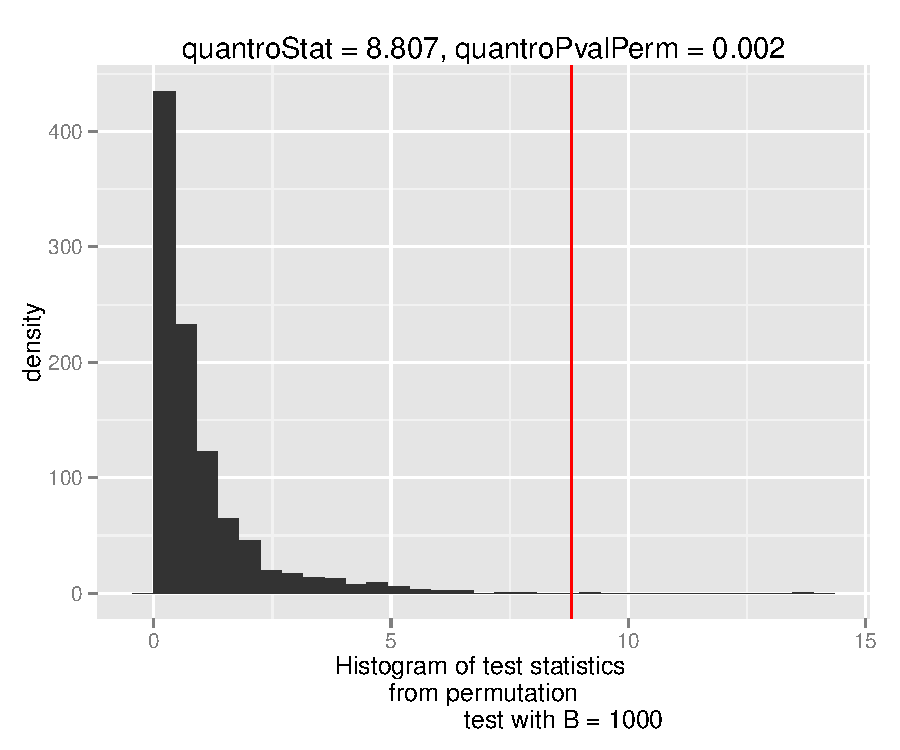
\includegraphics[width=\maxwidth]{figure/quantro-plot-1} 

\end{knitrout}


Additional options in the \texttt{quantroPlot()} function include:

\begin{table}[h]
\begin{center}
\begin{tabular}{|c|c|}
\hline
Element & Description \\
\hline
xLab & the x-axis label \\
yLab & the y-axis label \\
mainLab & title of the histogram \\
binWidth & change the binwidth \\
\hline
\end{tabular}
\end{center}
\label{tab:plots}
\end{table}


\section{SessionInfo}

\begin{knitrout}
\definecolor{shadecolor}{rgb}{0.969, 0.969, 0.969}\color{fgcolor}\begin{kframe}
\begin{alltt}
\hlkwd{sessionInfo}\hlstd{()}
\end{alltt}
\begin{verbatim}
## R version 3.1.3 (2015-03-09)
## Platform: x86_64-apple-darwin13.4.0 (64-bit)
## Running under: OS X 10.10.2 (Yosemite)
## 
## locale:
## [1] en_US.UTF-8/en_US.UTF-8/en_US.UTF-8/C/en_US.UTF-8/en_US.UTF-8
## 
## attached base packages:
## [1] stats4    parallel  stats     graphics  grDevices datasets  utils     methods  
## [9] base     
## 
## other attached packages:
##  [1] doParallel_1.0.8     minfi_1.12.0         bumphunter_1.6.0     locfit_1.5-9.1      
##  [5] iterators_1.0.7      foreach_1.4.2        Biostrings_2.34.1    XVector_0.6.0       
##  [9] GenomicRanges_1.18.4 GenomeInfoDb_1.2.4   IRanges_2.0.1        S4Vectors_0.4.0     
## [13] lattice_0.20-30      Biobase_2.26.0       BiocGenerics_0.12.1  quantro_1.1.2       
## [17] knitr_1.9           
## 
## loaded via a namespace (and not attached):
##  [1] annotate_1.44.0       AnnotationDbi_1.28.2  base64_1.1           
##  [4] beanplot_1.2          BiocStyle_1.4.1       codetools_0.2-11     
##  [7] colorspace_1.2-6      compiler_3.1.3        DBI_0.3.1            
## [10] digest_0.6.8          doRNG_1.6             evaluate_0.5.5       
## [13] formatR_1.0           genefilter_1.48.1     ggplot2_1.0.1        
## [16] grid_3.1.3            gtable_0.1.2          highr_0.4            
## [19] illuminaio_0.8.0      labeling_0.3          limma_3.22.7         
## [22] MASS_7.3-40           matrixStats_0.14.0    mclust_4.4           
## [25] multtest_2.22.0       munsell_0.4.2         nlme_3.1-120         
## [28] nor1mix_1.2-0         pkgmaker_0.22         plyr_1.8.1           
## [31] preprocessCore_1.28.0 proto_0.3-10          quadprog_1.5-5       
## [34] RColorBrewer_1.1-2    Rcpp_0.11.5           registry_0.2         
## [37] reshape_0.8.5         reshape2_1.4.1        rngtools_1.2.4       
## [40] RSQLite_1.0.0         scales_0.2.4          siggenes_1.40.0      
## [43] splines_3.1.3         stringr_0.6.2         survival_2.38-1      
## [46] tools_3.1.3           XML_3.98-1.1          xtable_1.7-4         
## [49] zlibbioc_1.12.0
\end{verbatim}
\end{kframe}
\end{knitrout}


\bibliography{library}


\end{document}
